\section{Failure Analysis}
\label{app:failure-analysis}

The appendix preserves negative and mixed evidence. Retained records include
schedule mismatch cases, solver adapter failures, teacher-alignment gains with
generation-metric degradation, CFG mismatch, NaN or empty scoring checks,
unstable timestep snapping, and settings where offline baselines remain
stronger than ours.

Current retained evidence includes PNDM rho/metric ablations, two failed
project-owned offline-proxy CIFAR diagnostics, and a matched SD1.5 CFG sweep. In
the SD1.5 Euler NFE-10 sweep, ours trails base and AYS on ImageReward
across CFG 5.0, 7.5, and 10.0 and gives no CLIPScore gain. This is a concrete
negative text-to-image case.

% Auto-generated by paper/figures/src/aggregate_failure_cases.py
\begin{table}[t]
\centering
\caption{Retained failure and sensitivity cases. Positive FID deltas are worse; negative ImageReward deltas are worse.}
\label{tab:failure-cases-summary}
\scriptsize
\setlength{\tabcolsep}{3pt}
\begin{tabular}{p{0.13\linewidth}p{0.21\linewidth}p{0.16\linewidth}p{0.13\linewidth}rp{0.15\linewidth}}
\toprule
Case & Setting & Comparison & Metric & Delta & Takeaway \\
\midrule
rho=0 geometry & PNDM/CIFAR-10 Euler, NFE 10, seed 0, 5k samples & ours rho=0 - base & FID (lower better) & +30.922 & Removing the residual mix makes FID much worse than base. \\
EDM scalar metric & PNDM/CIFAR-10 Euler, NFE 10, seed 0, 5k samples & ours EDM scalar - base & FID (lower better) & +4.871 & This metric variant loses the base-schedule gain. \\
Mean aggregation & PNDM/CIFAR-10 Euler, NFE 15, seed 0, 5k samples & mean - CVaR & FID (lower better) & +0.071 & Mean aggregation remains positive but trails CVaR. \\
SD1.5 CFG 5 & SD1.5 Euler, NFE 10, 3 seeds, 50 prompts per seed & ours - base & ImageReward (higher better) & -0.133 & Matched text-to-image calibration lowers ImageReward. \\
SD1.5 CFG 7.5 & SD1.5 Euler, NFE 10, 3 seeds, 50 prompts per seed & ours - base & ImageReward (higher better) & -0.084 & Matched text-to-image calibration lowers ImageReward. \\
SD1.5 CFG 10 & SD1.5 Euler, NFE 10, 3 seeds, 50 prompts per seed & ours - base & ImageReward (higher better) & -0.087 & Matched text-to-image calibration lowers ImageReward. \\
\bottomrule
\end{tabular}
\end{table}


\begin{table}[t]
  \centering
  \caption{Retained lightweight offline-proxy CIFAR-10 baseline.
  Rows report PNDM/CIFAR-10 Euler FID, mean $\pm$ standard error over
  seeds 0, 1, and 2 with 50k generated images per seed. The
  offline-proxy schedule is a small-budget project-owned hierarchical
  coordinate-search run, not the published AYS schedule. Lower FID is
  better.}
  \label{tab:cifar10-pndm-euler-50k-offline-proxy}
  \begin{tabular}{rrrrr}
    \toprule
    NFE & base & Karras & ours & offline-proxy \\
    \midrule
    10 & 20.57 $\pm$ 0.08 & 25.84 $\pm$ 0.10 & 17.54 $\pm$ 0.08 & 41.37 $\pm$ 0.13 \\
    20 & 11.17 $\pm$ 0.07 & 10.64 $\pm$ 0.09 & 10.71 $\pm$ 0.07 & 22.36 $\pm$ 0.05 \\
    \bottomrule
  \end{tabular}
\end{table}


Table~\ref{tab:cifar10-pndm-euler-50k-offline-proxy} records a failed
small-budget project-owned offline optimization attempt for PNDM/CIFAR-10. The
optimizer used the standalone hierarchical coordinate-search exporter with 256
training images and no FID proxy early stopping. It is not the published AYS
schedule. We retain it only as negative evidence because its FID is much worse
than base, Karras, and ours at both NFE values.

Before spending 50k samples on another failed schedule, we also ran a
higher-budget offline-proxy smoke diagnostic. The exporter used 1024 training
images, seven candidates per coordinate, FID proxy early stopping for the
10-step stage, and 5k FID evaluation over seeds 0--2. It reached
$26.76 \pm 0.06$ FID at NFE 10 and $18.32 \pm 0.03$ FID at NFE 20. These
values remain far outside the competitive range, so we keep the run as failure
evidence. The paper stores the cleaned diagnostic rows and optimizer config copy
under \texttt{paper/results/failure/}.

We also logged a pre-stage-bundle default-budget attempt with 8192 training
images and 11 candidates per coordinate. Its 10-step proxy FID increased from
31.9996 to 75.8249 over four iterations after the first best value, then the
20-step refinement stage remained slow before interruption. We therefore treat
that earlier run only as feasibility evidence for default-budget cost. The
later authorized offline run uses saved NFE 10 and 20 stage bundles and appears
in the main CIFAR table. The paper stores the cleaned one-row feasibility
record under \texttt{paper/results/failure/}.

Figure~\ref{fig:sd15-failure-grid} shows the three matched SD1.5 prompt/seed
pairs with the largest ImageReward drop for ours relative to the base
Euler schedule. The paper stores the selection metadata in
\texttt{paper/results/failure/sd15\_failure\_grid\_selection.csv}.

\begin{figure}[t]
  \centering
  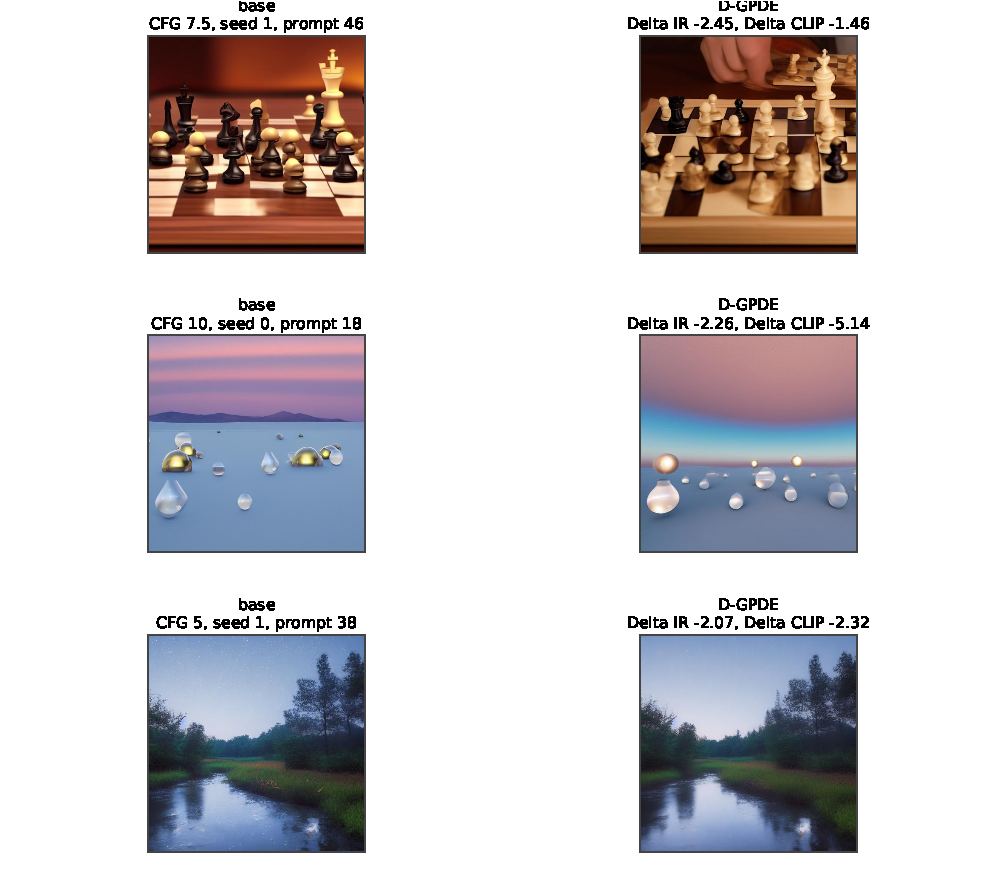
\includegraphics[width=\linewidth]{figures/sd15_failure_grid.pdf}
  \caption{Qualitative failure grid for the matched SD1.5 Euler NFE-10 CFG
  sweep. Each row compares the base schedule with ours for the same
  prompt, seed, and guidance scale. The cases are selected by the largest
  ours-minus-base ImageReward drop among retained matched samples.}
  \label{fig:sd15-failure-grid}
\end{figure}
